\begin{sidewaysfigure}[!htbp]
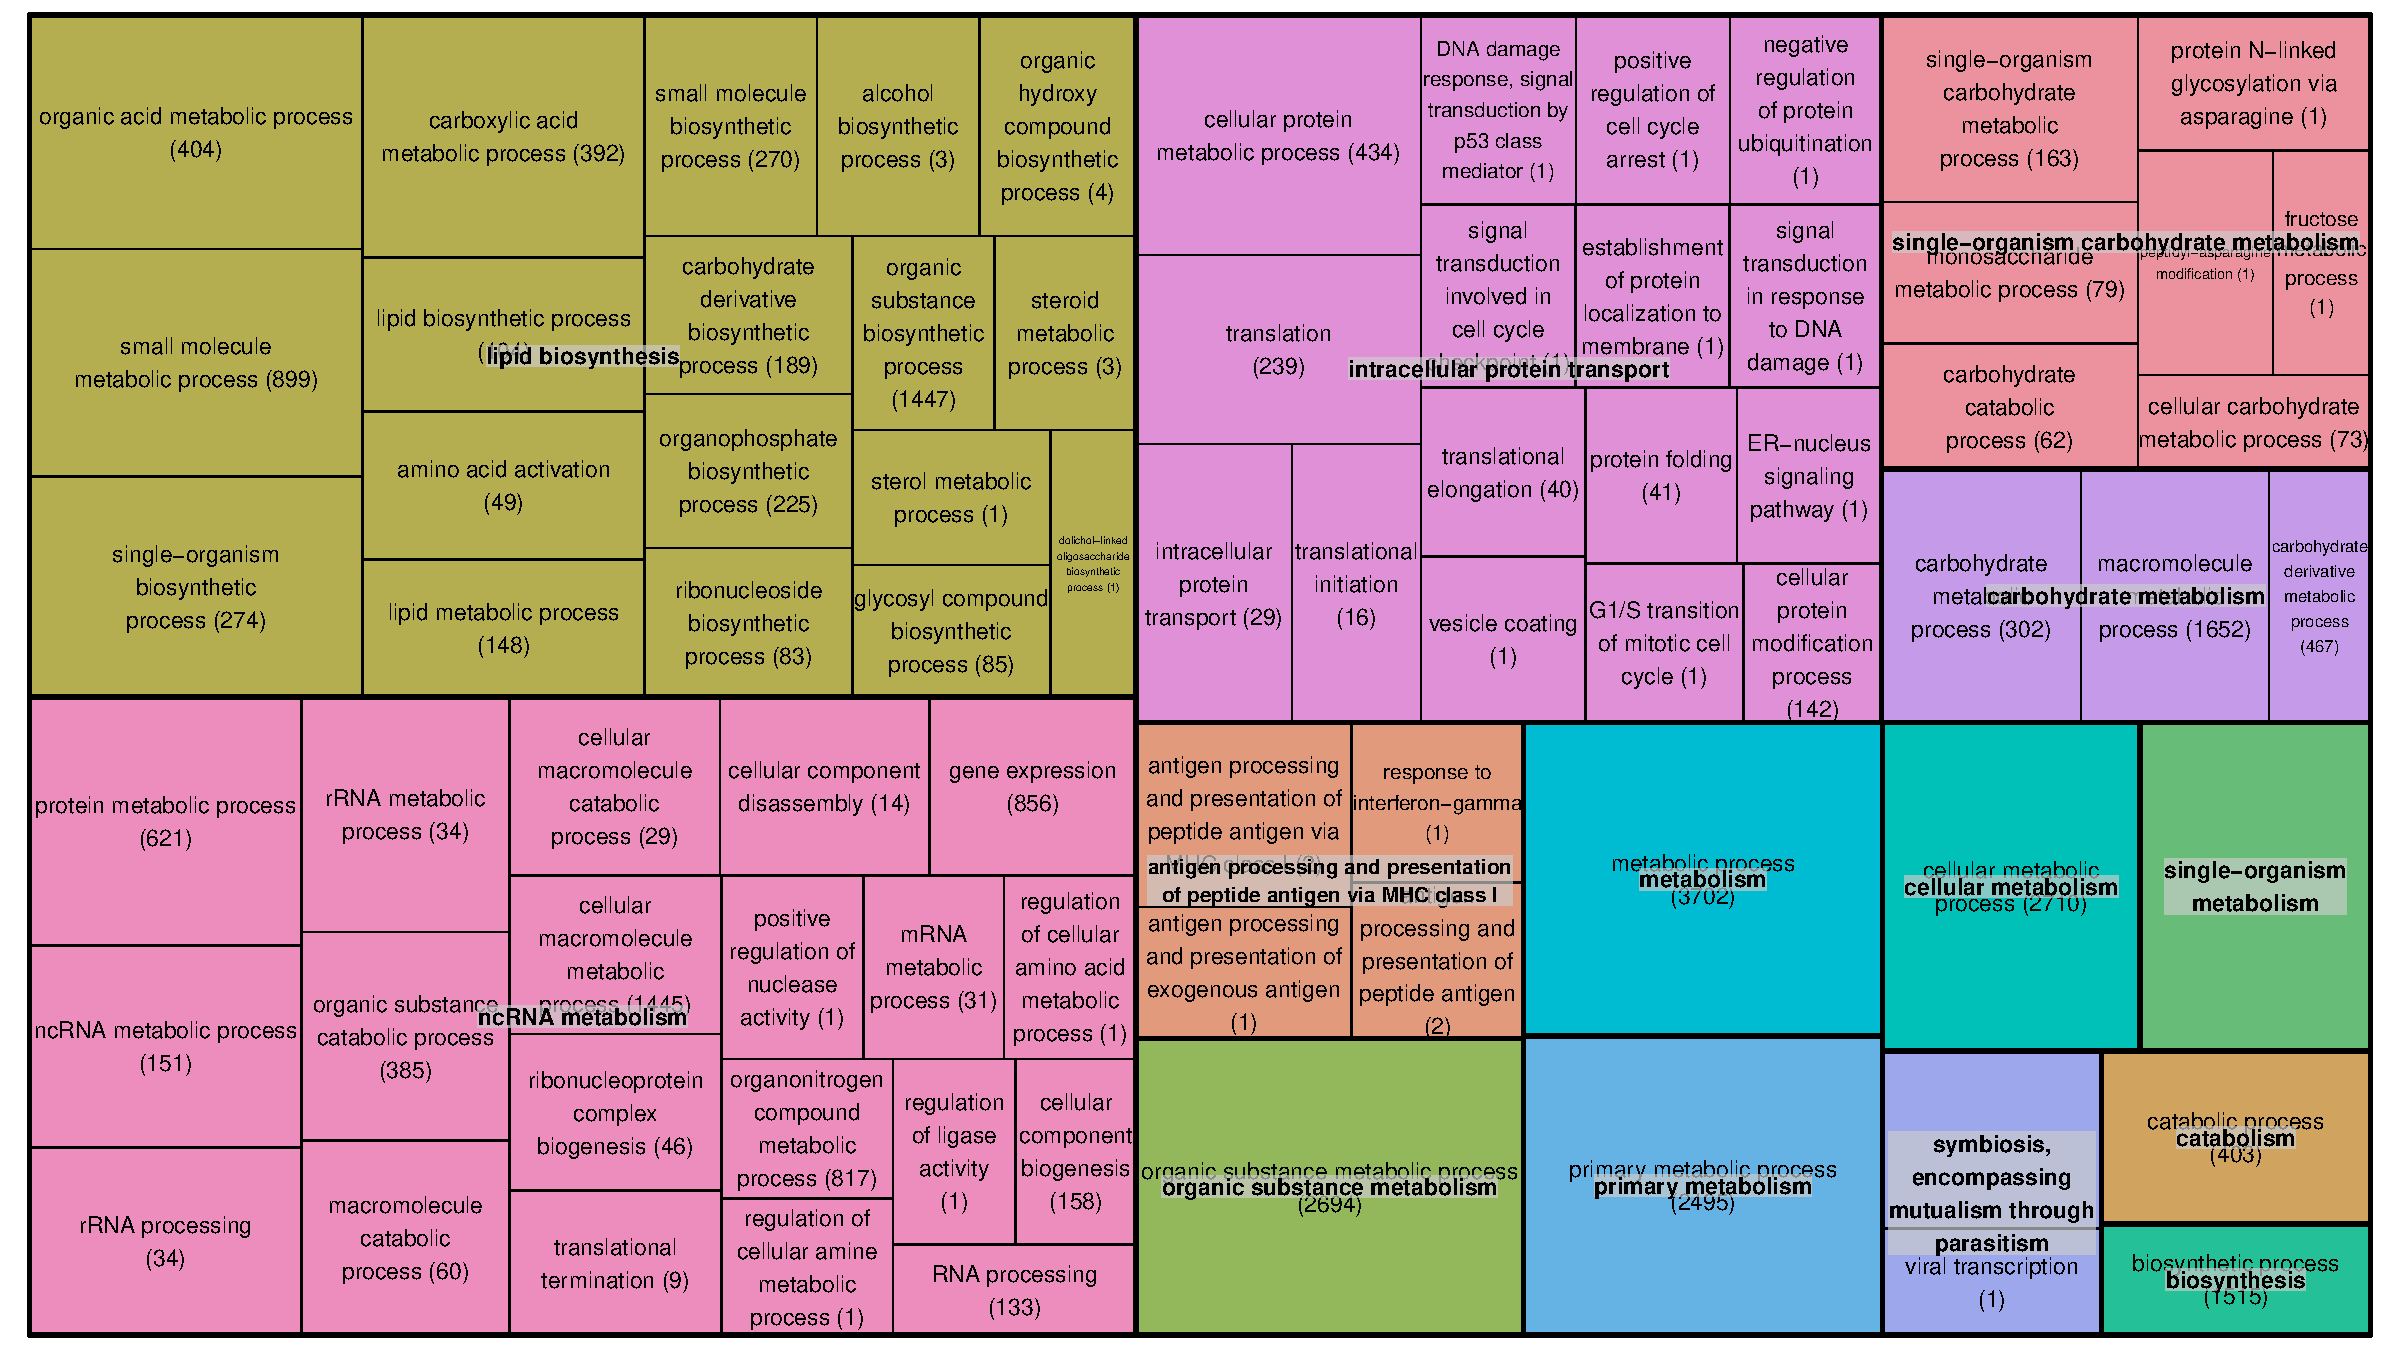
\includegraphics[width=\textwidth]
{Figures/hlc-go-all-treemap/hlc-go-all-treemap.pdf}
\caption[Enrichissement des catégories fonctionnelles associées aux gènes différentiellement exprimés dans les bourgeons de pattes postérieures]
{
Enrichissement des catégories fonctionnelles associées aux gènes différentiellement exprimés dans les bourgeons de pattes postérieures.
L'enrichissement de catégories fonctionnelles obtenu \autoref{fig:hlc-go-all-graph} a subit un post-traitement à l'aide de REViGO \citep{Supek2011} afin de résumer les différentes catégories avec une granularité moindre (deux niveaux) et de les représenter sous forme de "treemap".
La taille des rectangles est proportionnelle à la significativité de l'enrichissement de la catégorie fonctionnelle associée.
Le nombre de gènes associé à chaque catégorie est indiqué dans chaque cadre.
Un gène pouvant être associé à plusieurs catégories, le total du nombre de gènes indiqué dans chaque case est supérieur au nombre de gènes utilisé en entrée.
}
\label{fig:hlc-go-all-treemap}
\end{sidewaysfigure}